% !TeX root = ../Thesis.tex
\documentclass[../Thesis.tex]{subfiles}
\graphicspath{{\subfix{../images/}}}

\begin{document}

\section{Function inlining in the translation to Petri nets}

In this section, a concise analysis and motivation for the third design decision
listed at the beginning of the chapter, namely inlining function calls, is presented.

Modeling functions in \acrshort{PN} is a crucial aspect of the translation
because it is the basic unit of the MIR representation.
By representing the functions in the MIR as \acrshort{PN} and connecting them accordingly,
the control flow and data shared between the threads in the program
can be captured in a formal framework.
Afterward, the Petri net is analyzed by a model checker
in order to identify potential deadlocks or lost signals.
This approach is especially useful when working with large and complex systems
that may have many interrelated threads and functions,
where the deadlock situation may not be evident even to an experienced code reviewer.

When translating MIR functions to \acrshort{PN}, one key question that arises is
whether to reuse the same representation for every call to a specific function or
to ``inline'' the corresponding representation every time the function is called.
Expressed differently, each function maps to a subnet
in the final \acrshort{PN} obtained after the translation, i.e.
a connected subgraph formed by the places and transitions
that model the behavior of the specific function.
This smaller part of the net can either be present only once in the \acrshort{PN}
and all calls to this function connect to it,
or be repeated for every instance of a call to the function in the Rust code.

Reusing the same model for every function call can be more efficient,
as the \acrshort{PN} obtained is smaller.
However, this approach can also lead to invalid sequences of markings
that were not present in the original program.
These can be the source of false positives in deadlock detection,
as these extraneous states may lead the program to
incorrect states where the safety guarantees made by the compiler do not longer hold.

On the other hand, inlining the model every time a function is called results in
a larger \acrshort{PN}, which requires more memory and processor time to be analyzed,
but it can also improve the accuracy of the analysis by ensuring
that each function call is represented by a unique Petri net structure
that captures its specific data dependencies in the context
in which the function call occurs in the code.

The impact of these subtle details can only
be fully comprehended with an appropriate example.
Therefore, consider first the most simple abstraction of a function call in
the language of Petri nets, formed by a single transition and
two places representing the start and end of the function.
This is seen in Fig. \ref{fig:simplest-function}.
The function call is treated as a black box,
all details are abstracted away in the transition.
We care only about where the function starts and where it ends.

\begin{figure}[!htb]
    \centering
    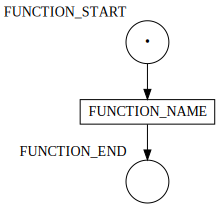
\includegraphics[scale=0.25]{simplest-function.png}
    \caption{The simplest Petri net model for a function call}
    \label{fig:simplest-function}
\end{figure}

Observe now such a function in the context of a Rust program.
Listing \ref{lst:repeated-function-call} shows a simple example
in which one function is called
five times consecutively in a \Rustinline{for} loop.
A possible \acrshort{PN} that models the program
is found in Fig. \ref{fig:repeated-function-call}.
It should be emphasized that
this net does \emph{not} result from a translation of the MIR.
It is a simplification to showcase the difficulties
of dealing with functions called in various places in the code.

\begin{listing}
    \begin{minted}{Rust}
        fn simple_function() {}

        pub fn main() {
            for i in 0..5 {
                simple_function();
            }
        }
    \end{minted}
    \caption{A simple Rust program with a repeated function call}
    \label{lst:repeated-function-call}
\end{listing}

\begin{figure}[!htb]
    \centering
    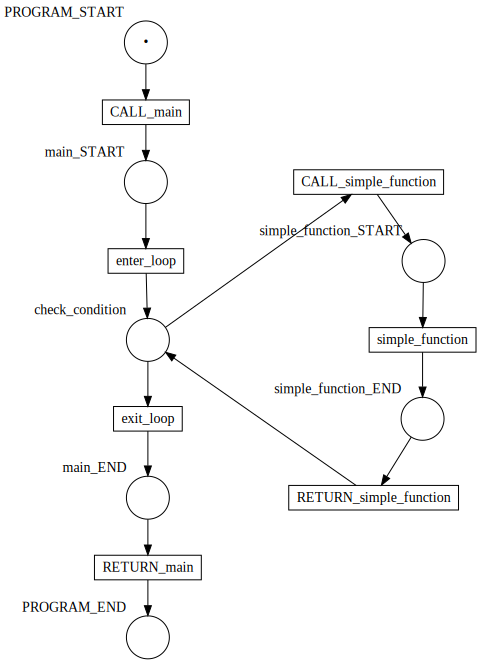
\includegraphics[scale=0.25]{repeated-function-call.png}
    \caption{A possible \acrshort{PN} for the code in Listing \ref{lst:repeated-function-call}
        which applies the model shown in Fig. \ref{fig:simplest-function}}
    \label{fig:repeated-function-call}
\end{figure}

\end{document}